\documentclass[en]{sdqbeamer} 

%Preamble
\usepackage{amssymb}
\usepackage{amsmath}
\usepackage[export]{adjustbox}
\usepackage[citestyle=numeric, bibstyle=numeric, backend=biber]{biblatex}
\addbibresource{../latex/References.bib}
\bibhang1em
\setbeamertemplate{bibliography item}{\insertbiblabel}

\newenvironment{rcases}
{\left.\begin{aligned}}
{\end{aligned}\right\rbrace}

%Title
\titleimage{banner_2020_kit}
\groupname{Research group for heterogeneous and parallel computing }
\title[Hardware Accelerators for Neural Networks]{A Survey on Hardware Accelerators for Neural Networks}
\author[Pierre Brosemer]{Pierre Brosemer}
\date[23.\,03.\,2020]{23. March 2020}

\begin{document}
	
\KITtitleframe

\begin{frame}{Table of contents}
\tableofcontents
\end{frame}

\section{Fundamentals neural networks}
\begin{frame}
	\begin{figure}
		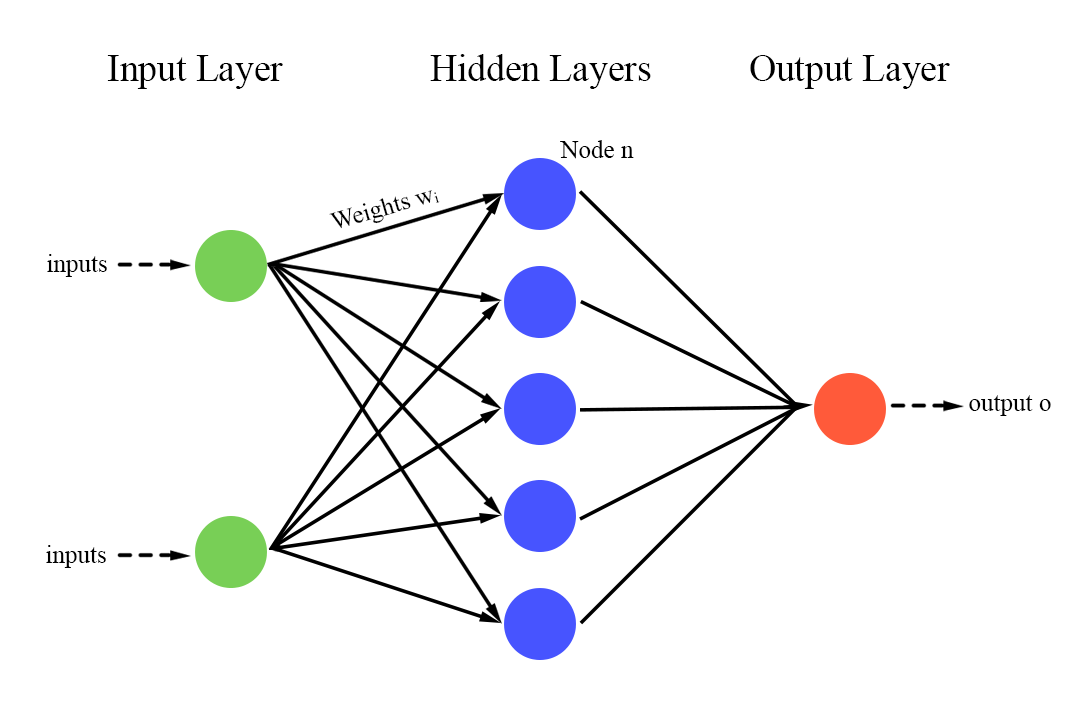
\includegraphics[width= 0.6\paperwidth]{pictures/neuralnetwork.png}
	\end{figure}
	\centering
	A typical representation of a neural network.
\end{frame}

\begin{frame}
	\begin{figure}
		\centering
		\begin{minipage}{0.45\paperwidth}
			\centering
			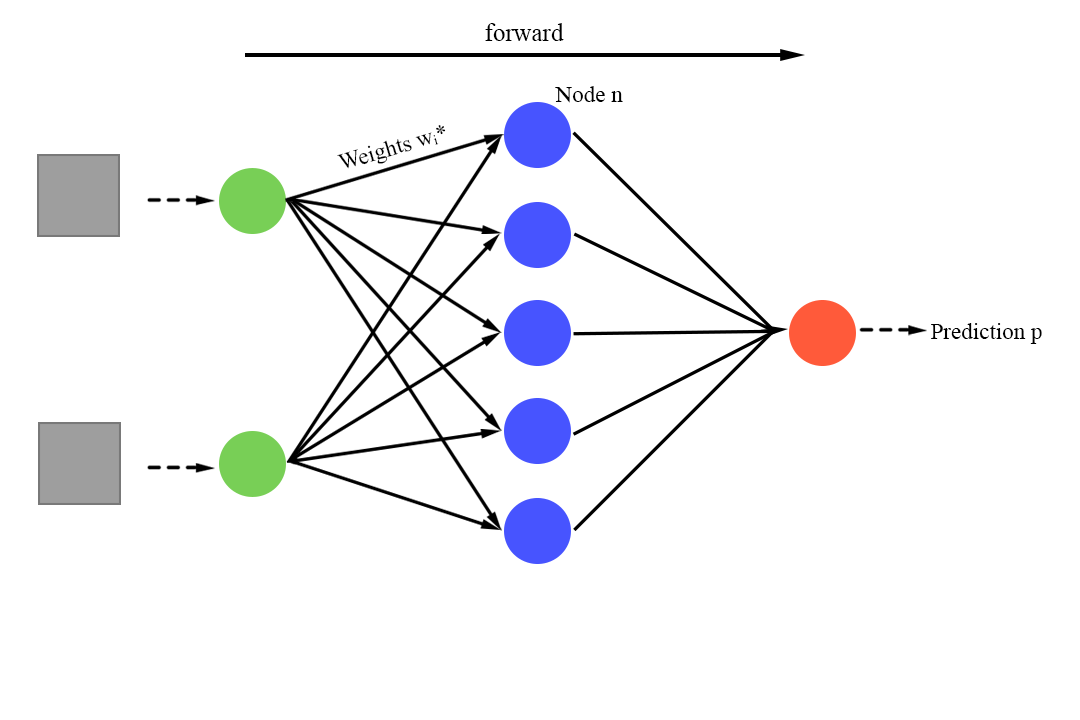
\includegraphics[width=0.45\paperwidth]{pictures/inference.png}
			\caption{Inference phase for a neural network}
		\end{minipage}\vrule{}
		\begin{minipage}{0.45\paperwidth}
			\centering
			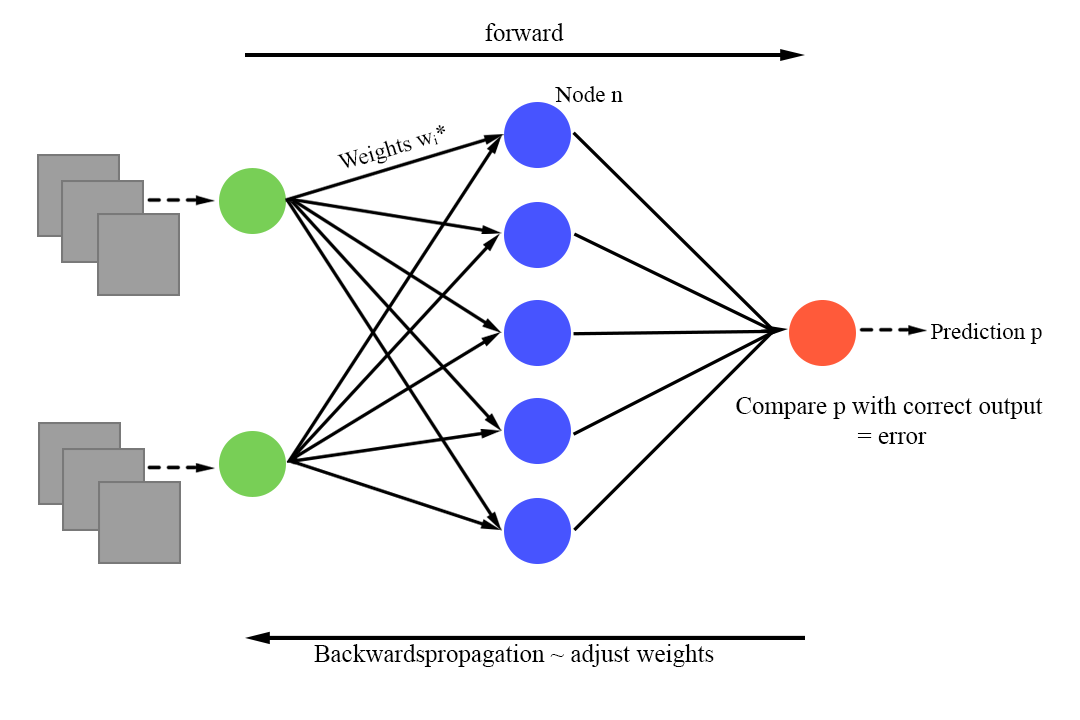
\includegraphics[width=0.45\paperwidth]{pictures/training.png}
			\caption{Training phase for a neural network}
		\end{minipage}
	\end{figure}
	$\rightsquigarrow$ vast amount of computational power
\end{frame}

\section{Different types of hardware}
\begin{frame}{Categorization}
Four main types:
\\
		\[
		\begin{rcases}
			\text{Central Processing Unit (CPU) } \\
			\text{Graphics Processing Unit (GPU) } 
		\end{rcases} \text{temporal architecture}
		\]
		\\
		\quad
		\\
		\[
		\begin{rcases}
			\text{Field-Programmable Gate Array (FPGA) } \\
			\text{Application-Specific Integrated Circuit (ASIC) }
		\end{rcases} \text{spatial architecture}
		\]
\end{frame}

\subsection{CPU}
\begin{frame}{Central Processing Unit}
	Properties of a CPU:
	\begin{itemize}
		\item good at executing serial instructions in parallel
		\item small amount of cores
		\item fetch instructions and execute
	\end{itemize}
	$\rightsquigarrow$ bad Parallelization for the same instruction\\ $\rightsquigarrow$ slow training and inference phases
\end{frame}

\subsection{GPU}
\begin{frame}{Graphics Processing Unit}
	\begin{minipage}[b]{0.45\paperwidth}
		Graphics Processing Unit
		\begin{itemize}
			\item specifications align with graphics rendering
			\item hundreds of cores with individual caches
			\item good parallelization of matrix multiplication
		\end{itemize}
	\end{minipage}
	\begin{minipage}{0.45\paperwidth}
		\begin{figure}
			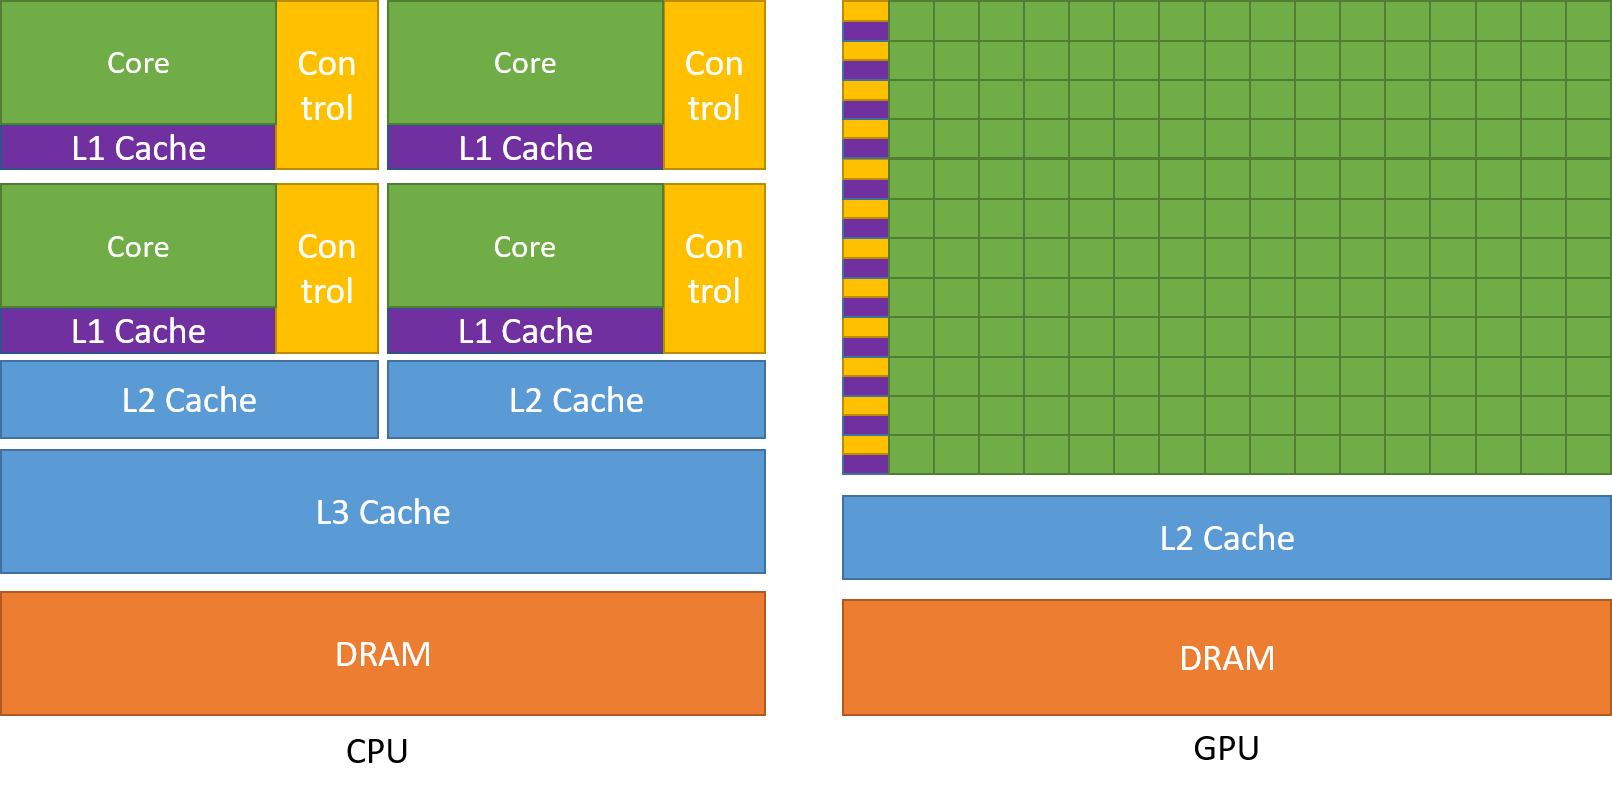
\includegraphics[width= 0.47\paperwidth, right]{pictures/intel_comparison.png}
			\caption{Layout differences between CPU and GPU \cite{intelpic_comparison}}
		\end{figure}
	\end{minipage}
\end{frame}

\begin{frame}{Acceleration by GPUs}
	Properties of GPUs for working with neural networks:
	\begin{itemize}
		\item achieve fast matrix multiplications
		\item make use of sparsity in matrices
		\item mostly used for training
		\item high memory bandwidth
	\end{itemize}
\end{frame}

\subsection{FPGA}
\begin{frame}{Field-Programmable Gate Array}
	General Properties:
	\begin{itemize}
		\item integrated circuit
		\item reprogramming with Hardware Description Language (HDL)
		\item limited flexibility compared to GPUs
		\item high compile times
	\end{itemize}
\end{frame}

\begin{frame}{Example speedup for a FPGA}
	Accelerating operation for recurrent neural networks \cite{nurvitadhi2016accelerating}:
	\begin{itemize}
		\item matrix divided into column blocks
		\item multiple FMA units
		\item each FMA unit responsible for one row in column block
		\item multiply rows to input vector
	\end{itemize}
\end{frame}

\begin{frame}
	\begin{figure}
		\centering
		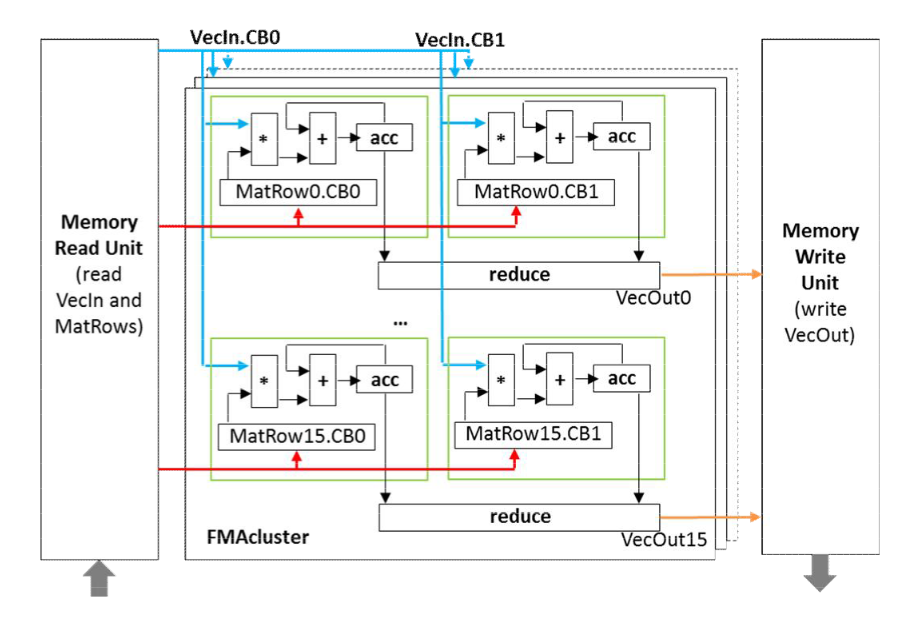
\includegraphics[width= 0.55\paperwidth]{pictures/fpga_operations.png}
		\caption{A simplified depiction showing the layout and dataflows of the previously mentioned FPGA \cite{nurvitadhi2016accelerating}}
	\end{figure}
\end{frame}

%Maybe Microsoft if enough Time

\subsection{ASIC}
\begin{frame}{Application-Specific Integrated Circuit}
	General Properties:
	\begin{itemize}
		\item integrated circuit
		\item can't be reprogrammed after production
		\item time-consuming and complicated process of design
		\item more energy-efficient than FPGAs
	\end{itemize}
\end{frame}

\begin{frame}
	
\end{frame}

\appendix
\beginbackup

\begin{frame}{References}
	\printbibliography
\end{frame}

\end{document}